\documentclass[t aspectratio=169]{beamer}
\usetheme{Rochester}
\usecolortheme{seahorse}
\usepackage{attachfile}
\usepackage{fontawesome5}
\usepackage{cmap}
\usepackage{mathtext}
\setbeamertemplate{footline}[frame number]
\usepackage[T2A]{fontenc}
\usepackage[utf8]{inputenc}
\usepackage[english,russian]{babel}
\title{Изучение методов фрактального сжатия для различных типов информации}
\author[author1]{Милов Данила Константинович\\[10mm]{\small Руководитель: Дудаков Сергей Михайлович}}
\begin{document}
  \begin{frame}
    \maketitle
  \end{frame}

  \section*{Оглавление}
  \begin{frame}\frametitle{\insertsection}
    \large
    \tableofcontents
    \normalfont
  \end{frame}

  \section{Актуальность работы}
  \begin{frame}\frametitle{\insertsection}
    \begin{columns}
      \column{0.5\textwidth}
      \begin{figure}
        \begin{center}
          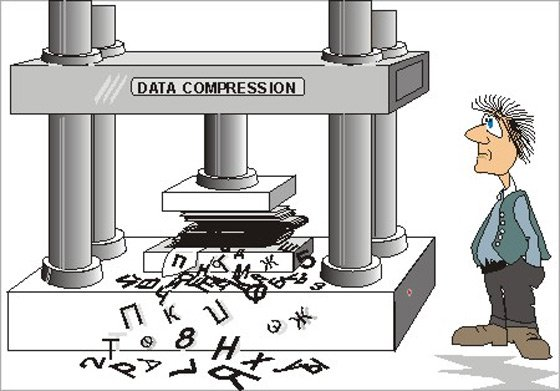
\includegraphics[width=1\textwidth]{./images/compression-illustration.jpg}
        \end{center}
      \end{figure}
      \column{0.5\textwidth}
      \large Необходимость сжатия информации
      \begin{itemize}
        \item Уменьшение занимаемого места на диске.
        \item Ускорение передачи данных за счёт меньшего объёма файлов.
        \item Более низкие затраты на хранение и пропускную способность.
      \end{itemize}
    \normalsize
    \end{columns}
  \end{frame}

  \section{Цели и задачи работы}
  \begin{frame}\frametitle{\insertsection}
    \large
    \begin{block}{Цель работы}
      Изучить и реализовать алгоритмы фрактального сжатия для различных типов информации
    \end{block}

    \vspace{0.5em}
    \textbf{Задачи}
    \begin{enumerate}
      \item Изучение алгоритмов фрактального сжатия для изображений.
      \item Изучение алгоритмов фрактального сжатия звука.
      \item Реализация алгоритмов фрактального сжатия.
      \item Сравнение качества сжимающих алгоритмов.
      \item Адаптация алгоритмов фрактального сжатия для других типов информации.
    \end{enumerate}
    \normalfont
  \end{frame}

  \section{Идея алгоритма}
  \begin{frame}\frametitle{\insertsection}
    \begin{figure}
      \begin{center}
        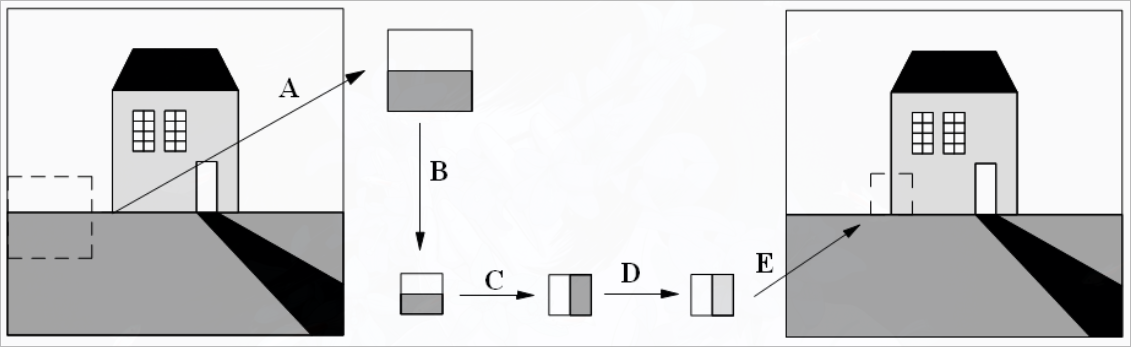
\includegraphics[width=\textwidth]{./images/algorithm-illustration.png}
      \end{center}
    \end{figure}
  \end{frame}

  \begin{frame}\frametitle{\insertsection}
    \large
    \begin{itemize}
      \item Метод разбиения.
      \item Метрика.
      \item Преобразования.
      \item Метод перебора.
      \item Декодирование.
      \item Хранение коэфициентов в файле.
    \end{itemize}
    \normalfont
  \end{frame}

  \begin{frame}\frametitle{Восстановление данных}
    \begin{figure}
      \begin{center}
        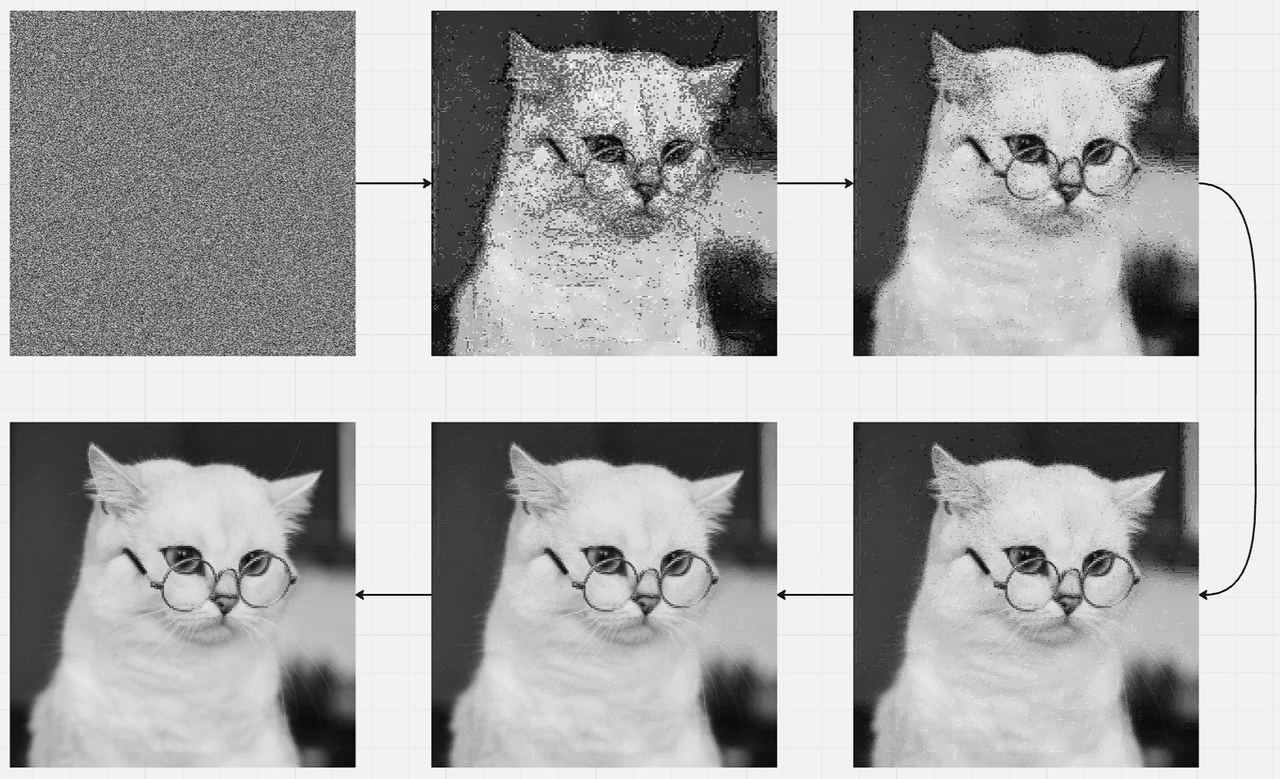
\includegraphics[width=\textwidth]{./images/cat_stages.jpg}
      \end{center}
    \end{figure}
  \end{frame}

  \begin{frame}\frametitle{Восстановление данных}
    \begin{figure}
      \begin{center}
        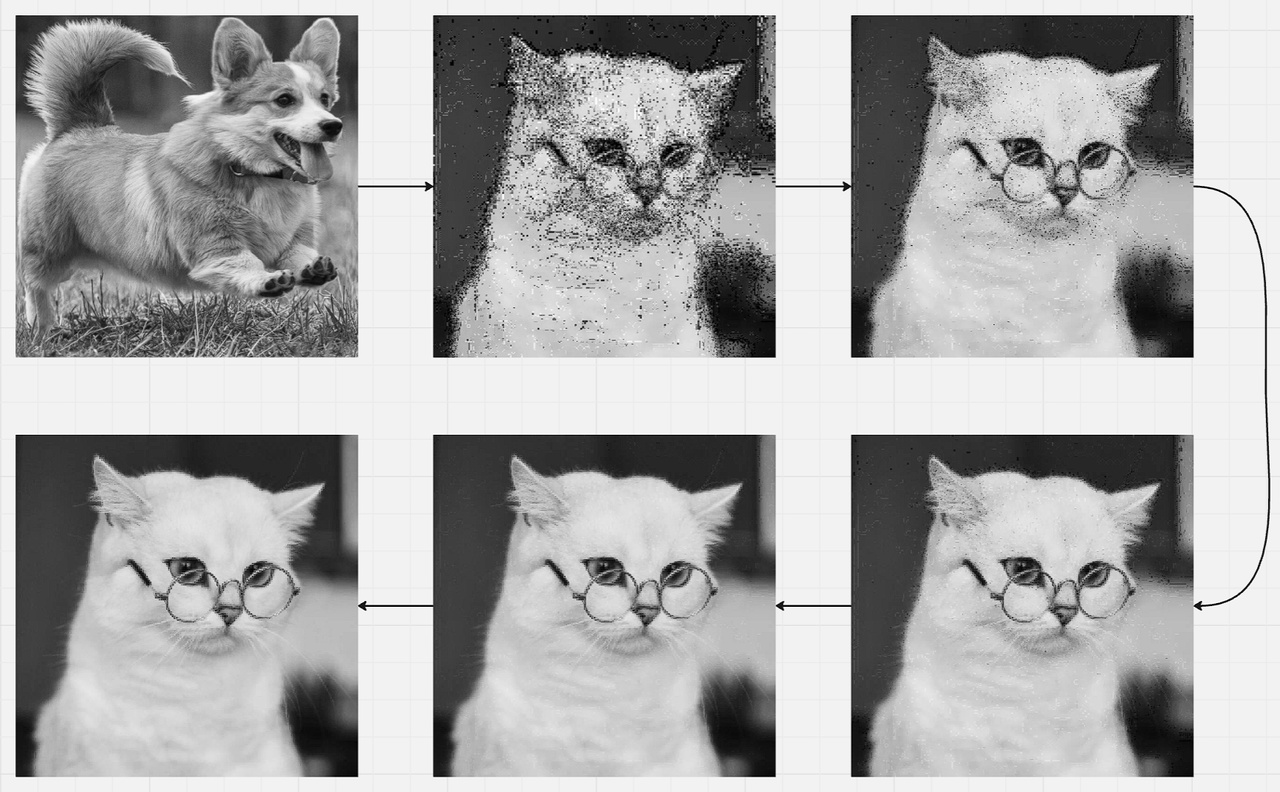
\includegraphics[width=\textwidth]{./images/cat_stages_dog.jpg}
      \end{center}
    \end{figure}
  \end{frame}


  \section{Результаты работы}

  \begin{frame}\frametitle{\insertsection . Изображения}
      \begin{figure}
        \begin{center}
          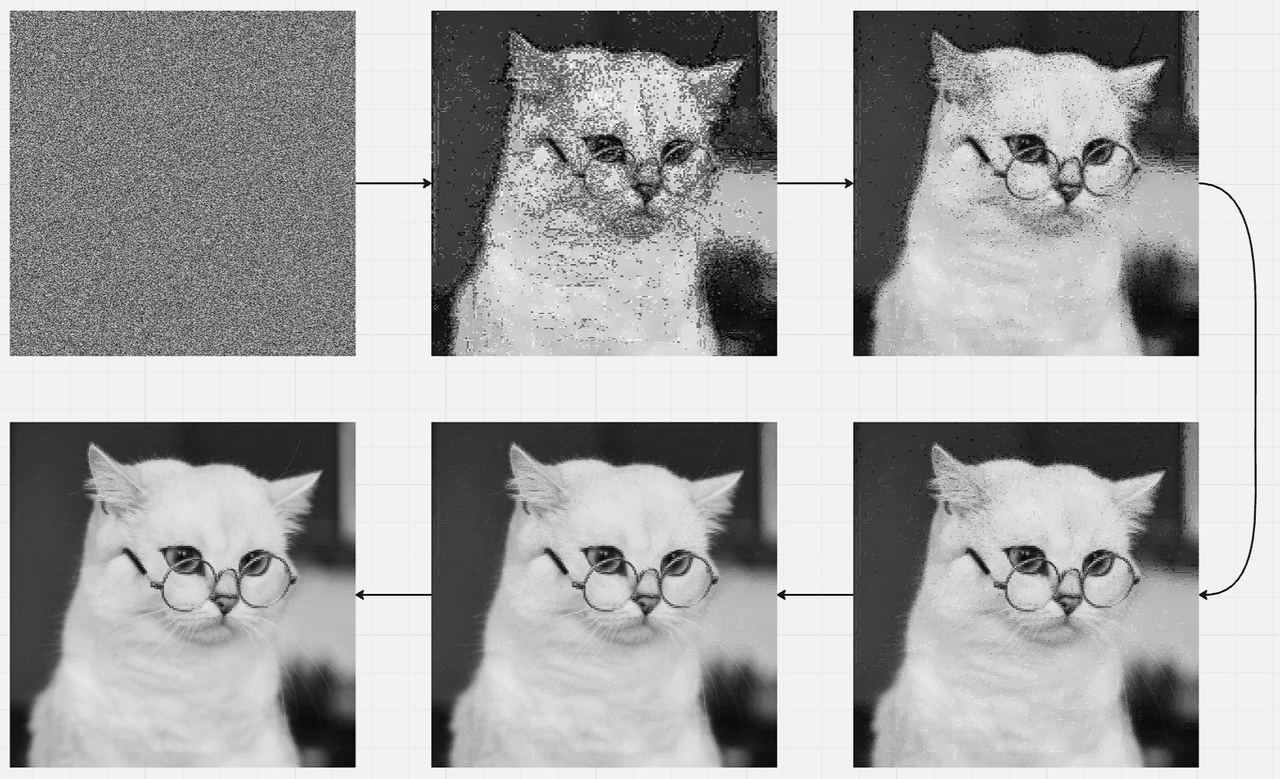
\includegraphics[width=1\textwidth]{./images/cat_stages.jpg}
        \end{center}
      \end{figure}
  \end{frame}

  \begin{frame}\frametitle{\insertsection . Изображения}
      \begin{figure}
        \begin{center}
          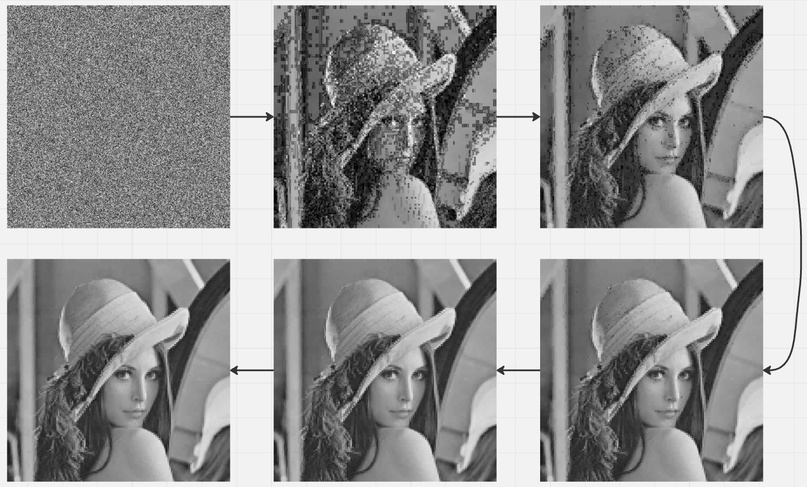
\includegraphics[width=1\textwidth]{./images/lena_stages.jpg}
        \end{center}
      \end{figure}
  \end{frame}

  \begin{frame}\frametitle{\insertsection . Изображения}
    \begin{columns}
      \column{0.5\textwidth}
      \large
      \begin{figure}
        \begin{center}
          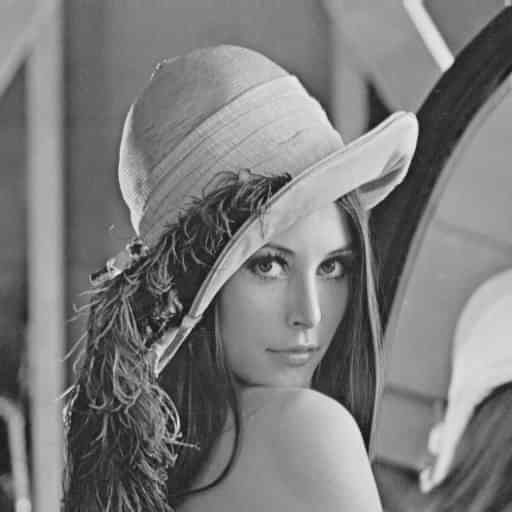
\includegraphics[width=1\textwidth]{./images/orig.png}
          \caption{Исходное изображение}
        \end{center}
      \end{figure}
      \column{0.5\textwidth}
      \begin{figure}
        \begin{center}
          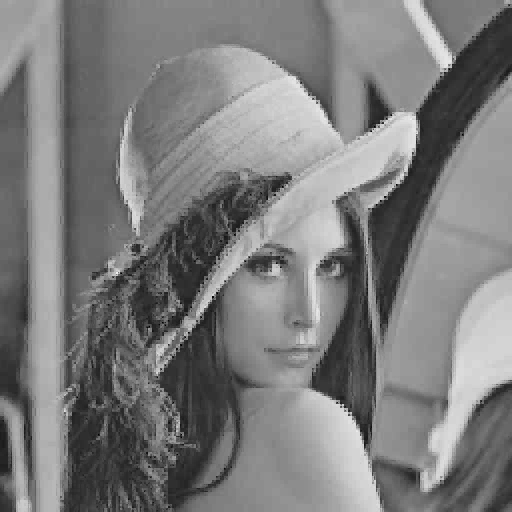
\includegraphics[width=1\textwidth]{./images/test.png}
          \caption{Результат алгоритма}
        \end{center}
      \end{figure}
    \normalsize
    \end{columns}
  \end{frame}

  \begin{frame}\frametitle{\insertsection . Изображения}
    \begin{columns}
      \column{0.5\textwidth}
      \large
      \begin{figure}
        \begin{center}
          
\includegraphics[width=1\textwidth]{./images/cat.png}
          \caption{Исходное изображение}
        \end{center}
      \end{figure}
      \column{0.5\textwidth}
      \begin{figure}
        \begin{center}
          
\includegraphics[width=1\textwidth]{./images/catr2.jpg}
          \caption{Результат алгоритма}
        \end{center}
      \end{figure}
    \normalsize
    \end{columns}
  \end{frame}

  \begin{frame}\frametitle{\insertsection . Аудиоданные}
      \begin{figure}
        \begin{center}
          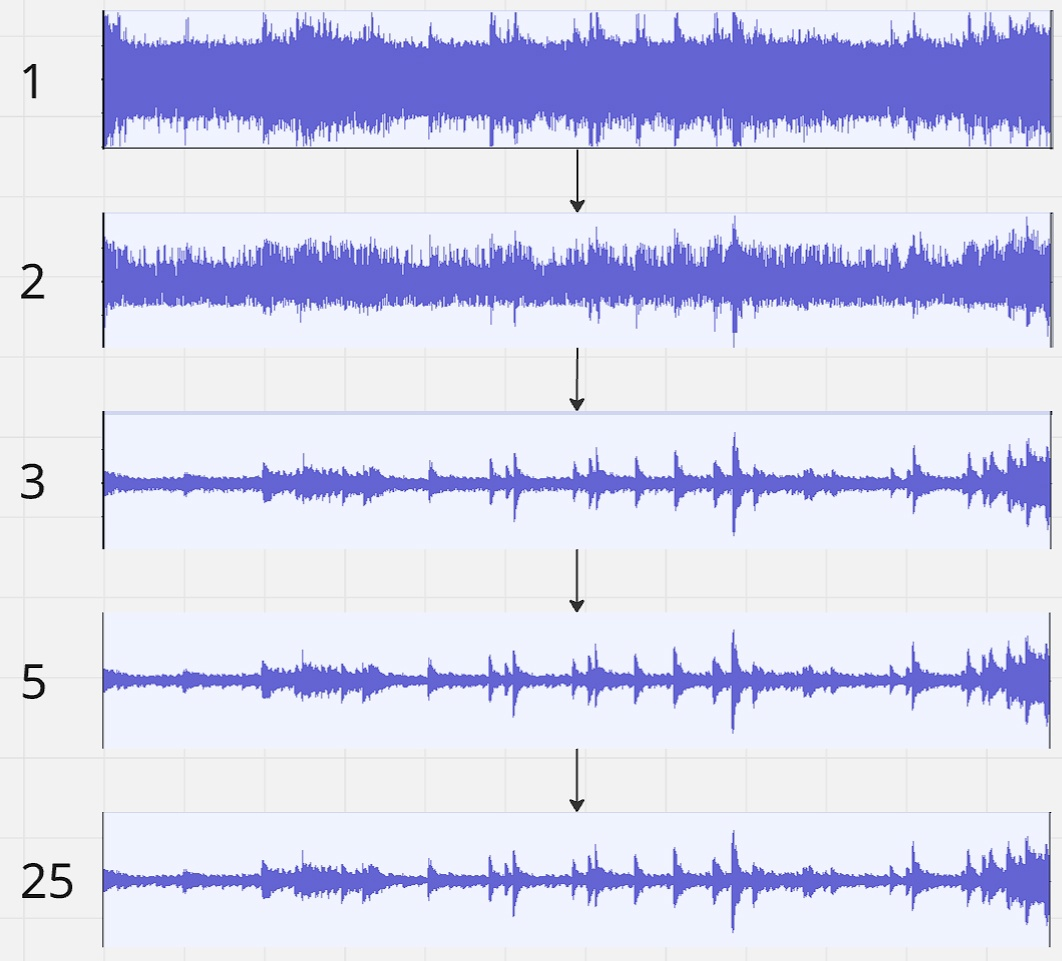
\includegraphics[width=0.7\textwidth]{./images/ms_stages.jpg}
        \end{center}
      \end{figure}
  \end{frame}

  \begin{frame}\frametitle{\insertsection . Аудиоданные}
      \begin{figure}
        \begin{center}
          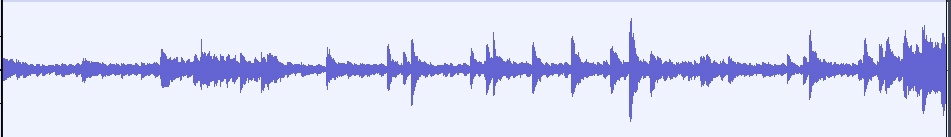
\includegraphics[width=1\textwidth]{./images/MS-init.jpg}
        \end{center}
        \caption{<<Лунная соната>>, исходные данные}
      \end{figure}

      \begin{figure}
        \begin{center}
          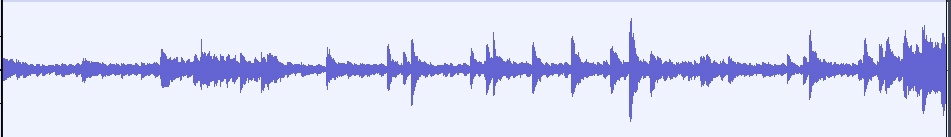
\includegraphics[width=1\textwidth]{./images/MS-init.jpg}
        \end{center}
        \caption{<<Лунная соната>>, восстановленные данные}
      \end{figure}
  \end{frame}

  \begin{frame}\frametitle{\insertsection . Аудиоданные}
      \begin{figure}
        \begin{center}
          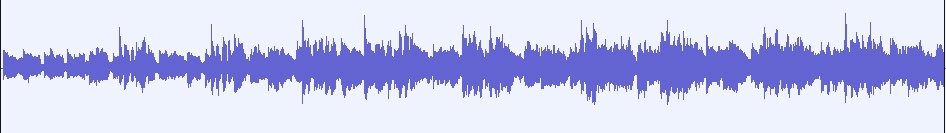
\includegraphics[width=1\textwidth]{./images/PBE-init.jpg}
        \end{center}
        \caption{<<Pale Blue Eyes>>, исходные данные}
      \end{figure}

      \begin{figure}
        \begin{center}
          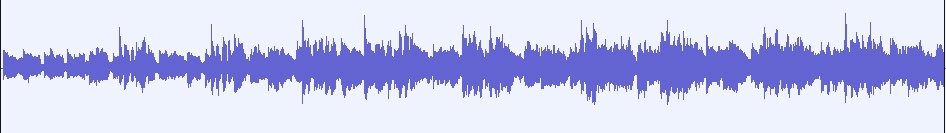
\includegraphics[width=1\textwidth]{./images/PBE-init.jpg}
        \end{center}
        \caption{<<Pale Blue Eyes>>, восстановленные данные}
      \end{figure}
  \end{frame}

  \begin{frame}\frametitle{\insertsection}
    \resizebox{\textwidth}{!}{
      \begin{tabular}{|c|c|c|c|}
        \hline
        Изображение, параметры & PSNR & К. сжатия & Время работы\\\hline
        cat 736$\times$736, r2d4 & 38dB & 0.75 & 35.4 с\\
        cat 736$\times$736, r4d8 & 42dB& 2.7 & 31.1 с \\
        cat 736$\times$736, r4d16 & 41dB & 2.7 & 18.7 с \\
        cat 736$\times$736, r8d16 & 43 dB & 11.5 & 11.6 с \\
        lena 512$\times$512, r2d4 & 30dB & 1.13 & 11.5 с \\
        lena 512$\times$512, r4d8 & 38dB & 4.76 & 9.8 с \\
        lena 512$\times$512, r4d16 & 35dB & 4.76 & 5.1 с \\
        lena 512$\times$512, r8d16 & 42dB & 20 & 3.2 с \\\hline
    \end{tabular}}
  \end{frame}

  \begin{frame}\frametitle{\insertsection}
    \resizebox{\textwidth}{!}{
    \begin{tabular}{|c|c|c|c|}
      \hline
      Аудио, параметры & PSNR & К. сжатия & Время работы\\\hline
      MS.wav, r4d8   & 32.4dB & 0.98 & 14 с\\
      MS.wav, r6d18  & 33.8dB & 1.47 & 45 с \\
      MS.wav, r10d20 & 35.6dB & 2.36 & 34 с \\
      MS.wav, r10d30 & 34dB   & 2.36 & 33.6 с \\
      PBE.wav, r2d4  & 31.3dB & 0.98 & 15 с \\
      PBE.wav, r4d8  & 34dB   & 1.47 & 47 с \\
      PBE.wav, r4d16 & 34.8dB & 2.36 & 32 с \\
      PBE.wav, r8d16 & 34.3dB & 2.36 & 33.5 с \\\hline
    \end{tabular}}
  \end{frame}

  \section{CLI-интерфейс программы}
  \begin{frame}\frametitle{\insertsection}
   \begin{figure}
    \begin{center}
      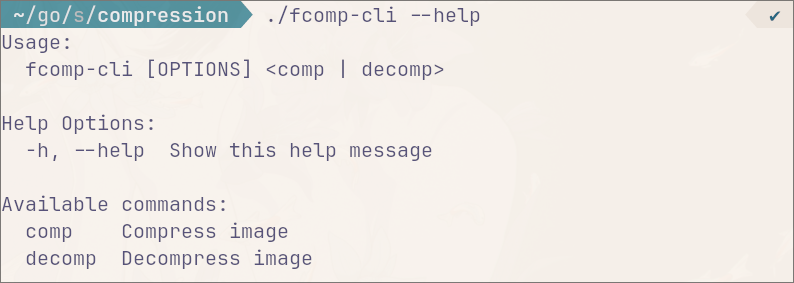
\includegraphics[width=\textwidth]{./images/cli-main.png}
    \end{center}
   \end{figure}
  \end{frame}

  \begin{frame}\frametitle{\insertsection. Команда comp}
   \begin{figure}
    \begin{center}
      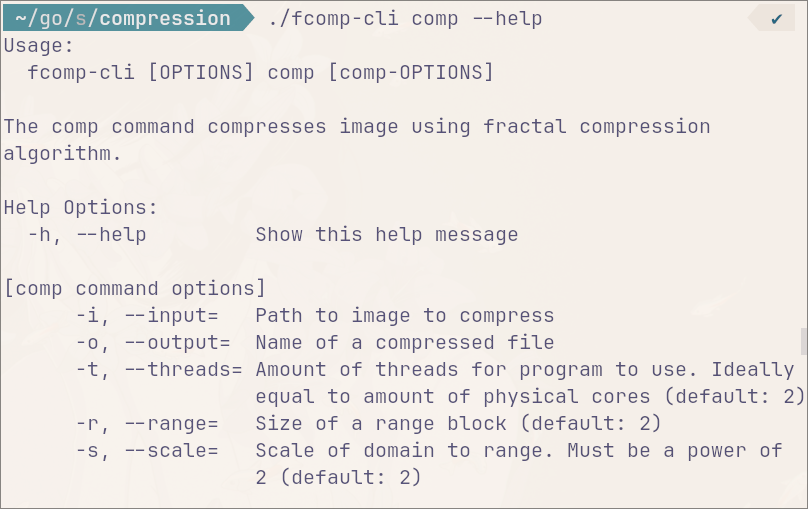
\includegraphics[width=\textwidth]{./images/cli-comp.png}
    \end{center}
   \end{figure}
  \end{frame}

  \begin{frame}\frametitle{\insertsection. Команда decomp}
   \begin{figure}
    \begin{center}
      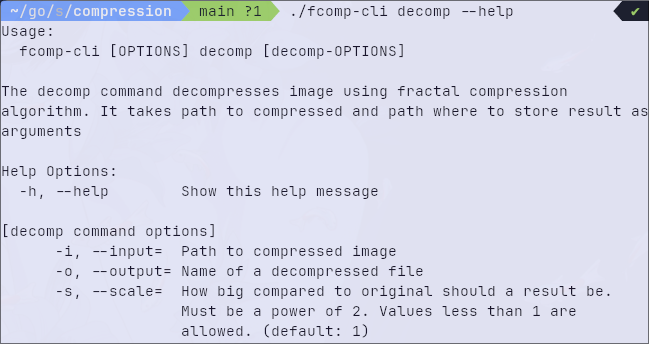
\includegraphics[width=\textwidth]{./images/cli-decomp.png}
    \end{center}
   \end{figure}
  \end{frame}

  \section{Заключение}
  \begin{frame}\frametitle{\insertsection}
    \large
    В ходе работы были изучены и запрограммированы методы фрактального сжатия изображений и звука. Среди дальнейших улучшений можно выделить следующие.
    \begin{enumerate}
      \item Увеличение коэфициента сжатия путём использования разбиения при помощи квадродерева.
      \item Оптимизации и эвристики, направленные на ускорение сжатия.
      \item Создание графического интерфейса, позволяющего удобно регулировать параметры и управлять процессом кодирования и декодирования.
    \end{enumerate}
    \normalfont
  \end{frame}

  \section*{Спасибо за внимание!}
  \begin{frame}
    \begin{center}
      \huge Спасибо за внимание!\normalfont
    \end{center}
  \end{frame}

\end{document}
